\documentclass[12pt,a4paper]{article}

\usepackage[a4paper,text={16.5cm,25.2cm},centering]{geometry}
\usepackage{lmodern}
\usepackage{amssymb,amsmath}
\usepackage{bm}
\usepackage{graphicx}
\usepackage{microtype}
\usepackage{hyperref}
\setlength{\parindent}{0pt}
\setlength{\parskip}{1.2ex}

\hypersetup
       {   pdfauthor = { David Kanter Eivin },
           pdftitle={ Pendulum Experiment },
           colorlinks=TRUE,
           linkcolor=black,
           citecolor=blue,
           urlcolor=blue
       }

\title{ Pendulum Experiment }

\author{ David Kanter Eivin }

\date{ 8th April 2022 }

\usepackage{upquote}
\usepackage{listings}
\usepackage{xcolor}
\lstset{
    basicstyle=\ttfamily\footnotesize,
    upquote=true,
    breaklines=true,
    breakindent=0pt,
    keepspaces=true,
    showspaces=false,
    columns=fullflexible,
    showtabs=false,
    showstringspaces=false,
    escapeinside={(*@}{@*)},
    extendedchars=true,
}
\newcommand{\HLJLt}[1]{#1}
\newcommand{\HLJLw}[1]{#1}
\newcommand{\HLJLe}[1]{#1}
\newcommand{\HLJLeB}[1]{#1}
\newcommand{\HLJLo}[1]{#1}
\newcommand{\HLJLk}[1]{\textcolor[RGB]{148,91,176}{\textbf{#1}}}
\newcommand{\HLJLkc}[1]{\textcolor[RGB]{59,151,46}{\textit{#1}}}
\newcommand{\HLJLkd}[1]{\textcolor[RGB]{214,102,97}{\textit{#1}}}
\newcommand{\HLJLkn}[1]{\textcolor[RGB]{148,91,176}{\textbf{#1}}}
\newcommand{\HLJLkp}[1]{\textcolor[RGB]{148,91,176}{\textbf{#1}}}
\newcommand{\HLJLkr}[1]{\textcolor[RGB]{148,91,176}{\textbf{#1}}}
\newcommand{\HLJLkt}[1]{\textcolor[RGB]{148,91,176}{\textbf{#1}}}
\newcommand{\HLJLn}[1]{#1}
\newcommand{\HLJLna}[1]{#1}
\newcommand{\HLJLnb}[1]{#1}
\newcommand{\HLJLnbp}[1]{#1}
\newcommand{\HLJLnc}[1]{#1}
\newcommand{\HLJLncB}[1]{#1}
\newcommand{\HLJLnd}[1]{\textcolor[RGB]{214,102,97}{#1}}
\newcommand{\HLJLne}[1]{#1}
\newcommand{\HLJLneB}[1]{#1}
\newcommand{\HLJLnf}[1]{\textcolor[RGB]{66,102,213}{#1}}
\newcommand{\HLJLnfm}[1]{\textcolor[RGB]{66,102,213}{#1}}
\newcommand{\HLJLnp}[1]{#1}
\newcommand{\HLJLnl}[1]{#1}
\newcommand{\HLJLnn}[1]{#1}
\newcommand{\HLJLno}[1]{#1}
\newcommand{\HLJLnt}[1]{#1}
\newcommand{\HLJLnv}[1]{#1}
\newcommand{\HLJLnvc}[1]{#1}
\newcommand{\HLJLnvg}[1]{#1}
\newcommand{\HLJLnvi}[1]{#1}
\newcommand{\HLJLnvm}[1]{#1}
\newcommand{\HLJLl}[1]{#1}
\newcommand{\HLJLld}[1]{\textcolor[RGB]{148,91,176}{\textit{#1}}}
\newcommand{\HLJLs}[1]{\textcolor[RGB]{201,61,57}{#1}}
\newcommand{\HLJLsa}[1]{\textcolor[RGB]{201,61,57}{#1}}
\newcommand{\HLJLsb}[1]{\textcolor[RGB]{201,61,57}{#1}}
\newcommand{\HLJLsc}[1]{\textcolor[RGB]{201,61,57}{#1}}
\newcommand{\HLJLsd}[1]{\textcolor[RGB]{201,61,57}{#1}}
\newcommand{\HLJLsdB}[1]{\textcolor[RGB]{201,61,57}{#1}}
\newcommand{\HLJLsdC}[1]{\textcolor[RGB]{201,61,57}{#1}}
\newcommand{\HLJLse}[1]{\textcolor[RGB]{59,151,46}{#1}}
\newcommand{\HLJLsh}[1]{\textcolor[RGB]{201,61,57}{#1}}
\newcommand{\HLJLsi}[1]{#1}
\newcommand{\HLJLso}[1]{\textcolor[RGB]{201,61,57}{#1}}
\newcommand{\HLJLsr}[1]{\textcolor[RGB]{201,61,57}{#1}}
\newcommand{\HLJLss}[1]{\textcolor[RGB]{201,61,57}{#1}}
\newcommand{\HLJLssB}[1]{\textcolor[RGB]{201,61,57}{#1}}
\newcommand{\HLJLnB}[1]{\textcolor[RGB]{59,151,46}{#1}}
\newcommand{\HLJLnbB}[1]{\textcolor[RGB]{59,151,46}{#1}}
\newcommand{\HLJLnfB}[1]{\textcolor[RGB]{59,151,46}{#1}}
\newcommand{\HLJLnh}[1]{\textcolor[RGB]{59,151,46}{#1}}
\newcommand{\HLJLni}[1]{\textcolor[RGB]{59,151,46}{#1}}
\newcommand{\HLJLnil}[1]{\textcolor[RGB]{59,151,46}{#1}}
\newcommand{\HLJLnoB}[1]{\textcolor[RGB]{59,151,46}{#1}}
\newcommand{\HLJLoB}[1]{\textcolor[RGB]{102,102,102}{\textbf{#1}}}
\newcommand{\HLJLow}[1]{\textcolor[RGB]{102,102,102}{\textbf{#1}}}
\newcommand{\HLJLp}[1]{#1}
\newcommand{\HLJLc}[1]{\textcolor[RGB]{153,153,119}{\textit{#1}}}
\newcommand{\HLJLch}[1]{\textcolor[RGB]{153,153,119}{\textit{#1}}}
\newcommand{\HLJLcm}[1]{\textcolor[RGB]{153,153,119}{\textit{#1}}}
\newcommand{\HLJLcp}[1]{\textcolor[RGB]{153,153,119}{\textit{#1}}}
\newcommand{\HLJLcpB}[1]{\textcolor[RGB]{153,153,119}{\textit{#1}}}
\newcommand{\HLJLcs}[1]{\textcolor[RGB]{153,153,119}{\textit{#1}}}
\newcommand{\HLJLcsB}[1]{\textcolor[RGB]{153,153,119}{\textit{#1}}}
\newcommand{\HLJLg}[1]{#1}
\newcommand{\HLJLgd}[1]{#1}
\newcommand{\HLJLge}[1]{#1}
\newcommand{\HLJLgeB}[1]{#1}
\newcommand{\HLJLgh}[1]{#1}
\newcommand{\HLJLgi}[1]{#1}
\newcommand{\HLJLgo}[1]{#1}
\newcommand{\HLJLgp}[1]{#1}
\newcommand{\HLJLgs}[1]{#1}
\newcommand{\HLJLgsB}[1]{#1}
\newcommand{\HLJLgt}[1]{#1}


\begin{document}

\maketitle


\section{Introduction}
Pendulums have for hundreds of years interested physics and industrialists alike. Not only are pendulums mystical to observe, they are immensely useful for mechanical timekeeping. From a physics standpoint, pendulums demonstrate the constant transformation between potential and kinetic energy, and, in a vacuum (with frictionless a frictionless pivot), can also demonstrate Newton's law of inertia by continuing to swing forever.

\begin{figure}
\centering
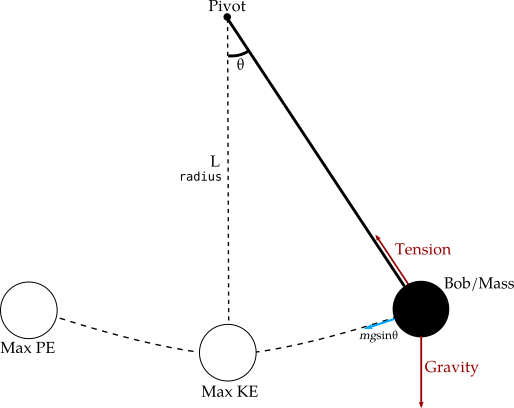
\includegraphics{pendulum.png}
\caption{Pendulum}
\end{figure}


Pendulums rely on the force of gravity pulling down on a massive bob, counteracted by tensive forces on the massless string/rod. The result is angular acceleration towards the point of maximum kinetic energy. An oscillation period is the time it takes for the bob to move across the pendulum (to the opposite point of maximum potential energy) and return to the highest point where it started.

This project simulates a pendulum and uses the results of the simulation to discuss the parameters determining a pendulum's period. The nature of a simulation means that while results are very precise and reproducible, their accuracy is largely dependent on previous observations: in this case, the laws of angular motion and air resistance. The code is included in this report is written in the simplest terms possible; while a software background may be helpful, a physics background should be sufficient to \emph{understand} the report \emph{and} the simulation's source code.

$\pagebreak$

\section{Purpose}
Given the importance of the oscillation period, this experiment examines the dependence of the period on the pendulum's \textbf{maximum/starting amplitude} and \textbf{length}. Additionally, the experiment aims to \textbf{precisely simulate pendulum movement} with and without air resistance for reuse in other pendulum experiments.

\section{Method}
\subsection{Software Simulation (Apparatus)}
The \href{https://julialang.org/}{Julia Programming Language} was selected for its readable mathematical syntax for non-technical readers and excellent performance. To avoid the tedious and unclear computation of kinetic vectors using $x$ and $y$ coordinates, I used Lagrangian mechanics to work directly with angular quantities. After deriving formulas for instantaneous angular acceleration ($\alpha$) and air resistance (shown below), I used Euler's method to compute the next angular velocity ($\omega$) and position ($\theta$). Essentially, angular acceleration is assumed to be constant for a small time interval $\Delta t$ in order to compute $\omega$. This is assumed to be constant for the same time interval, thus allowing the computation of $\theta$ at $t + \Delta t$. Time is then advanced by $\Delta t$ and $\theta$ is once again used to compute $\alpha$. \textbf{For all trials, $\Delta t = 0.0001\mathrm{s}$}. Each step is recorded into a \texttt{DataFrame} to be available for analysis and animation.

\subsubsection{Lagrangian}
The simulation formulas start from a general differential equation for motion.

\[
\frac{d}{dt} \frac{dL}{d\theta} = \frac{2L}{2\theta} - \frac{2D}{2\theta}
\]
where $L$ is the Lagrangian and $D$ is the dampening factor. Then, where $l$ represents the length of the rod:


\begin{align*}
    L &= K - U \\
    K &= \text{Kinetic Energy} = \frac{1}{2} mv^2 \\
    &= \frac{1}{2} ml^2\theta^2 \\ \\
    U &= \text{Potential Energy} = mgh = mg(l - l \cdot \cos \theta
\end{align*}
Together, this comprises the final Lagrangian:

\[
L = \frac{1}{2} ml^2\theta^2 - mg(l - l \cdot \cos \theta)
\]
which is differentiated with respect to $\theta$ to achieve:


\begin{align*}
    \frac{d}{dt}\left(ml^2\dot\theta\right) &= -L \sin\theta mg \\
    \implies \ddot\theta &= \alpha = -\frac{g\sin\theta}{l}
\end{align*}
As code:


\begin{lstlisting}
(*@\HLJLnf{dd\ensuremath{\theta}}@*)(*@\HLJLp{(}@*)(*@\HLJLn{\ensuremath{\theta}}@*)(*@\HLJLoB{::}@*)(*@\HLJLn{Number}@*)(*@\HLJLp{)}@*) (*@\HLJLoB{=}@*) (*@\HLJLoB{-}@*)(*@\HLJLp{(}@*)(*@\HLJLnf{sin}@*)(*@\HLJLp{(}@*)(*@\HLJLn{\ensuremath{\theta}}@*)(*@\HLJLp{)}@*) (*@\HLJLoB{*}@*) (*@\HLJLn{g}@*)(*@\HLJLp{)}@*) (*@\HLJLoB{/}@*) (*@\HLJLn{radius}@*)
\end{lstlisting}

\subsubsection{Air Resistance (drag)}
Using the above formula, this simulation will continue forever. While this is useful for studying theory, it will differ substantially from experimental results, which are impacted substantially by air resistance.

To simulate air resistance, first I determined whether the linear or quadratic formulas would be more appropriate.


\begin{align*}
\Omega_{\mathrm{linear}} &= bv = \ensuremath{\beta}Dv \\
\Omega_{\mathrm{quadratic}} &= cv^2 = \gamma D^2 v^2
\end{align*}
where $D$ is the diameter of the bob. The bob is assumed to be a sphere with $\gamma = 0.25$. I also chose to measure velocity from the point of maximum PE.


\begin{align*}
mgh &= \frac{1}{2} mv^2 \\
\implies gl &= v^2 \\
\implies v &= \sqrt{gl}
\end{align*}
Then:

\[
\frac{\Omega_{\mathrm{linear}}}{\Omega_{\mathrm{quadratic}}}
= \frac{\beta D \sqrt{gl}}{\gamma D^2 \sqrt{gl}^2}
= \frac{\beta}{\gamma D \sqrt{gl}}
\]
Using example values $D = 0.1\mathrm{m}$ and $l = 0.1\mathrm{m}$:


\begin{lstlisting}
(*@\HLJLp{(}@*)(*@\HLJLnfB{1.6e-4}@*)(*@\HLJLp{)}@*) (*@\HLJLoB{{\textbackslash}}@*) (*@\HLJLp{(}@*)(*@\HLJLn{\ensuremath{\gamma}}@*) (*@\HLJLoB{*}@*) (*@\HLJLn{D}@*) (*@\HLJLoB{*}@*) (*@\HLJLnf{sqrt}@*)(*@\HLJLp{(}@*)(*@\HLJLn{g}@*) (*@\HLJLoB{*}@*) (*@\HLJLn{l}@*)(*@\HLJLp{))}@*)
\end{lstlisting}

\begin{lstlisting}
154.75850643017978
\end{lstlisting}


we have that the quadratic formula is substantially larger (\texttt{{\textbackslash}} is \href{https://docs.julialang.org/en/v1/manual/mathematical-operations/#Arithmetic-Operators}{inverse division}) so \textbf{we will use the quadratic formula for air resistance}.

After differentiating and simplifying as we did previously, the formula for \ensuremath{\alpha} which accounts for drag is:

\[
\alpha = -\frac{g\sin\theta}{l} - \gamma D^2 l \omega^2
\]
Notably, this is \emph{not} a vector but a magnitude, and so direction must be adjusted to oppose $\omega$.


\begin{lstlisting}
(*@\HLJLnf{drag}@*)(*@\HLJLp{(}@*)(*@\HLJLn{\ensuremath{\omega}}@*)(*@\HLJLoB{::}@*)(*@\HLJLn{Number}@*)(*@\HLJLp{)}@*) (*@\HLJLoB{=}@*) (*@\HLJLn{\ensuremath{\gamma}}@*) (*@\HLJLoB{*}@*) (*@\HLJLp{(}@*)(*@\HLJLn{radius}@*)(*@\HLJLp{)}@*) (*@\HLJLoB{*}@*) (*@\HLJLp{(}@*)(*@\HLJLn{diameter}@*) (*@\HLJLoB{{\textasciicircum}}@*) (*@\HLJLni{2}@*)(*@\HLJLp{)}@*) (*@\HLJLoB{*}@*) (*@\HLJLp{(}@*)(*@\HLJLn{\ensuremath{\omega}}@*) (*@\HLJLoB{{\textasciicircum}}@*) (*@\HLJLni{2}@*)(*@\HLJLp{)}@*) (*@\HLJLoB{/}@*) (*@\HLJLn{mass}@*)
\end{lstlisting}

\subsubsection{Final Code:}
Using the above formulas, the iterative process for simulating data is summarized as follows (see Appendix A for full code).


\begin{lstlisting}
(*@\HLJLcs{{\#}}@*) (*@\HLJLcs{Initial}@*) (*@\HLJLcs{\ensuremath{\theta}}@*) (*@\HLJLcs{and}@*) (*@\HLJLcs{\ensuremath{\omega}}@*) (*@\HLJLcs{are}@*) (*@\HLJLcs{required.}@*)
(*@\HLJLcs{{\#}}@*) (*@\HLJLcs{\ensuremath{\theta}}@*) (*@\HLJLcs{is}@*) (*@\HLJLcs{provided}@*) (*@\HLJLcs{as}@*) (*@\HLJLcs{a}@*) (*@\HLJLcs{parameter,}@*) (*@\HLJLcs{\ensuremath{\omega}}@*) (*@\HLJLcs{is}@*) (*@\HLJLcs{assumed}@*) (*@\HLJLcs{to}@*) (*@\HLJLcs{be}@*) (*@\HLJLcs{0}@*)
(*@\HLJLn{\ensuremath{\omega}}@*) (*@\HLJLoB{=}@*) (*@\HLJLni{0}@*)
(*@\HLJLk{for}@*) (*@\HLJLn{t}@*) (*@\HLJLkp{in}@*) (*@\HLJLnf{range}@*)(*@\HLJLp{(}@*)(*@\HLJLni{0}@*)(*@\HLJLp{,}@*) (*@\HLJLn{duration}@*)(*@\HLJLp{;}@*) (*@\HLJLn{step}@*)(*@\HLJLoB{=}@*)(*@\HLJLn{\ensuremath{\Delta}t}@*)(*@\HLJLp{)}@*) (*@\HLJLcs{{\#}}@*) (*@\HLJLcs{increments}@*) (*@\HLJLcs{\ensuremath{\Delta}t}@*) (*@\HLJLcs{as}@*) (*@\HLJLcs{needed}@*)
    (*@\HLJLn{\ensuremath{\alpha}}@*) (*@\HLJLoB{=}@*) (*@\HLJLnf{dd\ensuremath{\theta}}@*)(*@\HLJLp{(}@*)(*@\HLJLn{\ensuremath{\theta}}@*)(*@\HLJLp{)}@*) (*@\HLJLoB{-}@*) (*@\HLJLnf{copysign}@*)(*@\HLJLp{(}@*)(*@\HLJLnf{drag}@*)(*@\HLJLp{(}@*)(*@\HLJLn{\ensuremath{\omega}}@*)(*@\HLJLp{),}@*) (*@\HLJLn{\ensuremath{\omega}}@*)(*@\HLJLp{)}@*)
    (*@\HLJLnf{push!}@*)(*@\HLJLp{(}@*)(*@\HLJLn{df}@*)(*@\HLJLp{,}@*) (*@\HLJLp{[}@*)(*@\HLJLn{t}@*)(*@\HLJLp{,}@*) (*@\HLJLn{\ensuremath{\theta}}@*)(*@\HLJLp{,}@*) (*@\HLJLn{\ensuremath{\omega}}@*)(*@\HLJLp{,}@*) (*@\HLJLn{\ensuremath{\alpha}}@*)(*@\HLJLp{])}@*) (*@\HLJLcs{{\#}}@*) (*@\HLJLcs{record}@*) (*@\HLJLcs{state}@*) (*@\HLJLcs{at}@*) (*@\HLJLcs{this}@*) (*@\HLJLcs{point}@*)
    (*@\HLJLn{\ensuremath{\omega}}@*) (*@\HLJLoB{+=}@*) (*@\HLJLn{\ensuremath{\alpha}}@*) (*@\HLJLoB{*}@*) (*@\HLJLn{\ensuremath{\Delta}t}@*)
    (*@\HLJLn{\ensuremath{\theta}}@*) (*@\HLJLoB{+=}@*) (*@\HLJLn{\ensuremath{\omega}}@*) (*@\HLJLoB{*}@*) (*@\HLJLn{\ensuremath{\Delta}t}@*)
(*@\HLJLk{end}@*)
\end{lstlisting}

\subsection{Data Collection}
To collect the relevant data, I first identified \& filtered for only the extremes of $\theta$ using $\omega$.


\begin{lstlisting}
(*@\HLJLk{function}@*) (*@\HLJLnf{extremes}@*)(*@\HLJLp{(}@*)(*@\HLJLn{df}@*)(*@\HLJLoB{::}@*)(*@\HLJLn{AbstractDataFrame}@*)(*@\HLJLp{)}@*)
    (*@\HLJLn{extremes}@*) (*@\HLJLoB{=}@*) (*@\HLJLnf{DataFrame}@*)(*@\HLJLp{(}@*)(*@\HLJLnf{first}@*)(*@\HLJLp{(}@*)(*@\HLJLn{df}@*)(*@\HLJLp{))}@*)
    (*@\HLJLk{for}@*) (*@\HLJLn{i}@*) (*@\HLJLkp{in}@*) (*@\HLJLni{3}@*)(*@\HLJLoB{:}@*)(*@\HLJLnf{nrow}@*)(*@\HLJLp{(}@*)(*@\HLJLn{df}@*)(*@\HLJLp{)}@*)
        (*@\HLJLk{if}@*) (*@\HLJLnf{sign}@*)(*@\HLJLp{(}@*)(*@\HLJLn{df}@*)(*@\HLJLp{[}@*)(*@\HLJLn{i}@*)(*@\HLJLoB{-}@*)(*@\HLJLni{1}@*)(*@\HLJLp{,}@*) (*@\HLJLsc{:\ensuremath{\omega}}@*)(*@\HLJLp{])}@*) (*@\HLJLoB{\ensuremath{\ne}}@*) (*@\HLJLnf{sign}@*)(*@\HLJLp{(}@*)(*@\HLJLn{df}@*)(*@\HLJLp{[}@*)(*@\HLJLn{i}@*)(*@\HLJLp{,}@*) (*@\HLJLsc{:\ensuremath{\omega}}@*)(*@\HLJLp{])}@*)
            (*@\HLJLnf{push!}@*)(*@\HLJLp{(}@*)(*@\HLJLn{extremes}@*)(*@\HLJLp{,}@*) (*@\HLJLn{df}@*)(*@\HLJLp{[}@*)(*@\HLJLn{i}@*)(*@\HLJLoB{-}@*)(*@\HLJLni{1}@*)(*@\HLJLp{,}@*) (*@\HLJLoB{:}@*)(*@\HLJLp{])}@*)
        (*@\HLJLk{end}@*)
    (*@\HLJLk{end}@*)
    (*@\HLJLn{extremes}@*)
(*@\HLJLk{end}@*)
\end{lstlisting}

The first period is then taken as the difference between the 1st and 3rd extreme.

The simulation is run several times with different parameters to simulate the independent variables under study (amplitude, length/radius), and the period is recorded at each step. Average period is taken as the mean of the first 15 periods (arbitrarily chosen).

In order to run the simulation with and without air resistance, I simply set $\gamma = 0$ which removes this term from the equation for $\alpha$.

\section{Results}
\subsection{General/Simulation Effectiveness}
Firstly, to validate our simulation for future tests, we can visualize the trajectory of our pendulum with and without air resistance.


\begin{lstlisting}
(*@\HLJLn{p}@*) (*@\HLJLoB{=}@*) (*@\HLJLnf{Pendulum}@*)(*@\HLJLp{(}@*)
    (*@\HLJLnfB{.3}@*)(*@\HLJLp{,}@*) (*@\HLJLcs{{\#}}@*) (*@\HLJLcs{30cm}@*) (*@\HLJLcs{pendulum}@*)
    (*@\HLJLnf{deg2rad}@*)(*@\HLJLp{(}@*)(*@\HLJLni{45}@*)(*@\HLJLp{),}@*) (*@\HLJLcs{{\#}}@*) (*@\HLJLcs{initial}@*) (*@\HLJLcs{\ensuremath{\theta}}@*)
    (*@\HLJLnf{Bob}@*)(*@\HLJLp{(}@*)
        (*@\HLJLn{mass}@*) (*@\HLJLoB{=}@*) (*@\HLJLnfB{.05}@*)(*@\HLJLp{,}@*) (*@\HLJLcs{{\#}}@*) (*@\HLJLcs{50g}@*)
        (*@\HLJLn{diameter}@*) (*@\HLJLoB{=}@*) (*@\HLJLnfB{.05}@*)(*@\HLJLp{,}@*) (*@\HLJLcs{{\#}}@*) (*@\HLJLcs{5cm}@*)
        (*@\HLJLn{\ensuremath{\gamma}}@*) (*@\HLJLoB{=}@*) (*@\HLJLn{\ensuremath{\gamma}}@*)
    (*@\HLJLp{)}@*)
(*@\HLJLp{)}@*)

(*@\HLJLn{with{\_}resistance}@*) (*@\HLJLoB{=}@*) (*@\HLJLnf{simulate}@*)(*@\HLJLp{(}@*)(*@\HLJLn{p}@*)(*@\HLJLp{,}@*) (*@\HLJLni{10}@*)(*@\HLJLp{)}@*)
(*@\HLJLn{no{\_}resistance}@*) (*@\HLJLoB{=}@*) (*@\HLJLnf{simulate}@*)(*@\HLJLp{(}@*)(*@\HLJLn{p}@*)(*@\HLJLp{,}@*) (*@\HLJLni{10}@*)(*@\HLJLp{,}@*) (*@\HLJLn{resistance}@*)(*@\HLJLoB{=}@*)(*@\HLJLkc{false}@*)(*@\HLJLp{)}@*)

(*@\HLJLnf{plot}@*)(*@\HLJLp{(}@*)
    (*@\HLJLn{with{\_}resistance}@*)(*@\HLJLp{[}@*)(*@\HLJLoB{!}@*)(*@\HLJLp{,}@*) (*@\HLJLsc{:time}@*)(*@\HLJLp{],}@*)
    (*@\HLJLp{[}@*)(*@\HLJLn{with{\_}resistance}@*)(*@\HLJLp{[}@*)(*@\HLJLoB{!}@*)(*@\HLJLp{,}@*) (*@\HLJLsc{:\ensuremath{\theta}}@*)(*@\HLJLp{],}@*) (*@\HLJLn{no{\_}resistance}@*)(*@\HLJLp{[}@*)(*@\HLJLoB{!}@*)(*@\HLJLp{,}@*) (*@\HLJLsc{:\ensuremath{\theta}}@*)(*@\HLJLp{]],}@*)
    (*@\HLJLn{label}@*) (*@\HLJLoB{=}@*) (*@\HLJLp{[}@*)(*@\HLJLs{"{}}@*)(*@\HLJLse{{\textbackslash}{\textbackslash}}@*)(*@\HLJLs{gamma}@*) (*@\HLJLs{=}@*) (*@\HLJLsi{{\$}\ensuremath{\gamma}}@*)(*@\HLJLs{"{}}@*) (*@\HLJLs{"{}}@*)(*@\HLJLse{{\textbackslash}{\textbackslash}}@*)(*@\HLJLs{gamma}@*) (*@\HLJLs{=}@*) (*@\HLJLs{0"{}}@*)(*@\HLJLp{],}@*)
    (*@\HLJLn{xlabel}@*) (*@\HLJLoB{=}@*) (*@\HLJLs{"{}Time}@*) (*@\HLJLs{(s)"{}}@*)(*@\HLJLp{,}@*)
    (*@\HLJLn{ylabel}@*) (*@\HLJLoB{=}@*) (*@\HLJLs{"{}Position}@*) (*@\HLJLs{(deg)"{}}@*)(*@\HLJLp{,}@*)
    (*@\HLJLn{yformatter}@*) (*@\HLJLoB{=}@*) (*@\HLJLn{round}@*) (*@\HLJLoB{\ensuremath{\circ}}@*) (*@\HLJLn{rad2deg}@*)
(*@\HLJLp{)}@*)
\end{lstlisting}

\includegraphics[width=\linewidth]{jl_dxD5vJ/report_7_1.pdf}

We can see that the pendulum in a vacuum has constant amplitude, whereas the simulation with air resistance displays a slight dampening effect. This effect is likely so pronounced because the bob is light (50.0g).

\subsection{Amplitude and Period}
As we can see from the below figure, as amplitude increases, the time of the first period (roughly equivalent to the period in a vacuum) increases as well. This effect is very minor below $30^\circ$ but becomes very pronounced above {\textasciitilde}80 degrees. The ability to simulate such high angles with "rod-like" behaviour (that is, with no flexibility in the string), is one advantage of using a computer simulation over a physical pendulum. While the average period also increases with amplitude, this effect is far less pronounced given that an increased velocity increases the dampening factor of air resistance. This curve is closer to what we would likely see in a real-life experiment on Earth.


\begin{lstlisting}
(*@\HLJLn{df}@*) (*@\HLJLoB{=}@*) (*@\HLJLnf{DataFrame}@*)(*@\HLJLp{(}@*)(*@\HLJLn{amplitude}@*)(*@\HLJLoB{=}@*)(*@\HLJLn{Number}@*)(*@\HLJLp{[],}@*) (*@\HLJLn{period{\_}initial}@*)(*@\HLJLoB{=}@*)(*@\HLJLn{Number}@*)(*@\HLJLp{[],}@*) (*@\HLJLn{period{\_}average}@*)(*@\HLJLoB{=}@*)(*@\HLJLn{Number}@*)(*@\HLJLp{[])}@*)

(*@\HLJLk{for}@*) (*@\HLJLn{deg}@*) (*@\HLJLkp{in}@*) (*@\HLJLnf{range}@*)(*@\HLJLp{(}@*)(*@\HLJLni{5}@*)(*@\HLJLp{,}@*) (*@\HLJLni{175}@*)(*@\HLJLp{;}@*) (*@\HLJLn{step}@*) (*@\HLJLoB{=}@*) (*@\HLJLni{2}@*)(*@\HLJLp{)}@*)
    (*@\HLJLkd{local}@*) (*@\HLJLn{p}@*) (*@\HLJLoB{=}@*) (*@\HLJLnf{Pendulum}@*)(*@\HLJLp{(}@*)(*@\HLJLnfB{.3}@*)(*@\HLJLp{,}@*) (*@\HLJLnf{deg2rad}@*)(*@\HLJLp{(}@*)(*@\HLJLn{deg}@*)(*@\HLJLp{),}@*) (*@\HLJLnf{Bob}@*)(*@\HLJLp{(}@*)(*@\HLJLnfB{.05}@*)(*@\HLJLp{,}@*) (*@\HLJLnfB{.05}@*)(*@\HLJLp{,}@*) (*@\HLJLn{\ensuremath{\gamma}}@*)(*@\HLJLp{))}@*)
    (*@\HLJLn{runthrough}@*) (*@\HLJLoB{=}@*) (*@\HLJLnf{simulate}@*)(*@\HLJLp{(}@*)(*@\HLJLn{p}@*)(*@\HLJLp{,}@*) (*@\HLJLni{30}@*)(*@\HLJLp{)}@*) (*@\HLJLoB{|>}@*) (*@\HLJLn{extremes}@*) (*@\HLJLoB{|>}@*) (*@\HLJLn{periods}@*)
    (*@\HLJLnd{@inbounds}@*) (*@\HLJLnf{push!}@*)(*@\HLJLp{(}@*)(*@\HLJLn{df}@*)(*@\HLJLp{,}@*) (*@\HLJLp{[}@*)(*@\HLJLn{deg}@*) (*@\HLJLn{runthrough}@*)(*@\HLJLp{[}@*)(*@\HLJLni{1}@*)(*@\HLJLp{]}@*) (*@\HLJLnf{mean}@*)(*@\HLJLp{(}@*)(*@\HLJLn{runthrough}@*)(*@\HLJLp{[}@*)(*@\HLJLni{1}@*)(*@\HLJLoB{:}@*)(*@\HLJLnf{min}@*)(*@\HLJLp{(}@*)(*@\HLJLni{20}@*)(*@\HLJLp{,}@*) (*@\HLJLnf{length}@*)(*@\HLJLp{(}@*)(*@\HLJLn{runthrough}@*)(*@\HLJLp{))])])}@*)
(*@\HLJLk{end}@*)

(*@\HLJLnf{plot}@*)(*@\HLJLp{(}@*)
    (*@\HLJLn{df}@*)(*@\HLJLp{[}@*)(*@\HLJLoB{!}@*)(*@\HLJLp{,}@*) (*@\HLJLsc{:amplitude}@*)(*@\HLJLp{],}@*)
    (*@\HLJLp{[}@*)(*@\HLJLn{df}@*)(*@\HLJLp{[}@*)(*@\HLJLoB{!}@*)(*@\HLJLp{,}@*) (*@\HLJLsc{:period{\_}initial}@*)(*@\HLJLp{]}@*) (*@\HLJLn{df}@*)(*@\HLJLp{[}@*)(*@\HLJLoB{!}@*)(*@\HLJLp{,}@*) (*@\HLJLsc{:period{\_}average}@*)(*@\HLJLp{]],}@*)
    (*@\HLJLn{label}@*) (*@\HLJLoB{=}@*) (*@\HLJLp{[}@*)(*@\HLJLs{"{}First}@*) (*@\HLJLs{Period"{}}@*) (*@\HLJLs{"{}Average}@*) (*@\HLJLs{Period"{}}@*)(*@\HLJLp{],}@*)
    (*@\HLJLn{xlabel}@*) (*@\HLJLoB{=}@*) (*@\HLJLs{"{}Amplitude}@*) (*@\HLJLs{(deg)"{}}@*)(*@\HLJLp{,}@*)
    (*@\HLJLn{ylabel}@*) (*@\HLJLoB{=}@*) (*@\HLJLs{"{}Period}@*) (*@\HLJLs{(s)"{}}@*)
(*@\HLJLp{)}@*)
\end{lstlisting}

\begin{figure}[!h]
\center
\includegraphics[width=\linewidth]{jl_dxD5vJ/report_8_1.pdf}
\caption{Oscillation period increases with release amplitude.}
\end{figure}

Showing the every 2 degrees of the first {\textasciitilde}20 extremes gives a close up of the effect on small angles.



\begin{tabular}{r|ccc}
	& amplitude & period\_initial & period\_average\\
	\hline
	& Number & Number & Number\\
	\hline
	1 & 5.0 & 1.0992 & 1.09928 \\
	2 & 7.0 & 1.0997 & 1.09977 \\
	3 & 9.0 & 1.1004 & 1.10041 \\
	4 & 11.0 & 1.1012 & 1.10121 \\
	5 & 13.0 & 1.1023 & 1.10215 \\
	6 & 15.0 & 1.1034 & 1.10326 \\
	7 & 17.0 & 1.1048 & 1.1045 \\
	8 & 19.0 & 1.1063 & 1.10589 \\
	9 & 21.0 & 1.108 & 1.10742 \\
	10 & 23.0 & 1.1098 & 1.10909 \\
	11 & 25.0 & 1.1119 & 1.1109 \\
	12 & 27.0 & 1.1141 & 1.11285 \\
	13 & 29.0 & 1.1165 & 1.11494 \\
	14 & 31.0 & 1.1191 & 1.11715 \\
	15 & 33.0 & 1.1218 & 1.1195 \\
	16 & 35.0 & 1.1247 & 1.12199 \\
	17 & 37.0 & 1.1279 & 1.1246 \\
	18 & 39.0 & 1.1312 & 1.12735 \\
	19 & 41.0 & 1.1347 & 1.13021 \\
	20 & 43.0 & 1.1384 & 1.13322 \\
\end{tabular}


\begin{figure}[!h]
\center
\includegraphics[width=\linewidth]{jl_dxD5vJ/report_10_1.pdf}
\caption{Period of First 20 Extremes: Detailed Image of Small Max Amplitudes.}
\end{figure}

This supports Galileo's hypothesis that amplitude has minimal/negligible impact on period at very small angles, but as angle increases, it starts to show very relevant effects.

\subsection{Length (radius) and Period}
Period also increase substantially as length is increased, from 10cm to 2m, though the rate of increase slows as the pendulum lengthens.


\begin{lstlisting}
(*@\HLJLn{df}@*) (*@\HLJLoB{=}@*) (*@\HLJLnf{DataFrame}@*)(*@\HLJLp{(}@*)(*@\HLJLn{len}@*)(*@\HLJLoB{=}@*)(*@\HLJLn{Number}@*)(*@\HLJLp{[],}@*) (*@\HLJLn{period{\_}initial}@*)(*@\HLJLoB{=}@*)(*@\HLJLn{Number}@*)(*@\HLJLp{[],}@*) (*@\HLJLn{period{\_}average}@*)(*@\HLJLoB{=}@*)(*@\HLJLn{Number}@*)(*@\HLJLp{[])}@*)

(*@\HLJLk{for}@*) (*@\HLJLn{len}@*) (*@\HLJLkp{in}@*) (*@\HLJLnf{range}@*)(*@\HLJLp{(}@*)(*@\HLJLnfB{.1}@*)(*@\HLJLp{,}@*) (*@\HLJLni{2}@*)(*@\HLJLp{,}@*) (*@\HLJLn{step}@*)(*@\HLJLoB{=}@*)(*@\HLJLnfB{.1}@*)(*@\HLJLp{)}@*)
    (*@\HLJLkd{local}@*) (*@\HLJLn{p}@*) (*@\HLJLoB{=}@*) (*@\HLJLnf{Pendulum}@*)(*@\HLJLp{(}@*)(*@\HLJLn{len}@*)(*@\HLJLp{,}@*) (*@\HLJLnf{deg2rad}@*)(*@\HLJLp{(}@*)(*@\HLJLni{30}@*)(*@\HLJLp{),}@*) (*@\HLJLnf{Bob}@*)(*@\HLJLp{(}@*)(*@\HLJLnfB{.05}@*)(*@\HLJLp{,}@*) (*@\HLJLnfB{.05}@*)(*@\HLJLp{,}@*) (*@\HLJLn{\ensuremath{\gamma}}@*)(*@\HLJLp{))}@*)
    (*@\HLJLn{runthrough}@*) (*@\HLJLoB{=}@*) (*@\HLJLnf{simulate}@*)(*@\HLJLp{(}@*)(*@\HLJLn{p}@*)(*@\HLJLp{,}@*) (*@\HLJLni{30}@*)(*@\HLJLp{)}@*) (*@\HLJLoB{|>}@*) (*@\HLJLn{extremes}@*) (*@\HLJLoB{|>}@*) (*@\HLJLn{periods}@*)
    (*@\HLJLnd{@inbounds}@*) (*@\HLJLnf{push!}@*)(*@\HLJLp{(}@*)(*@\HLJLn{df}@*)(*@\HLJLp{,}@*) (*@\HLJLp{[}@*)(*@\HLJLn{len}@*) (*@\HLJLn{runthrough}@*)(*@\HLJLp{[}@*)(*@\HLJLni{1}@*)(*@\HLJLp{]}@*) (*@\HLJLnf{mean}@*)(*@\HLJLp{(}@*)(*@\HLJLn{runthrough}@*)(*@\HLJLp{[}@*)(*@\HLJLni{1}@*)(*@\HLJLoB{:}@*)(*@\HLJLnf{min}@*)(*@\HLJLp{(}@*)(*@\HLJLni{20}@*)(*@\HLJLp{,}@*) (*@\HLJLnf{length}@*)(*@\HLJLp{(}@*)(*@\HLJLn{runthrough}@*)(*@\HLJLp{))])])}@*)
(*@\HLJLk{end}@*)

(*@\HLJLnf{plot}@*)(*@\HLJLp{(}@*)
    (*@\HLJLn{df}@*)(*@\HLJLp{[}@*)(*@\HLJLoB{!}@*)(*@\HLJLp{,}@*) (*@\HLJLsc{:len}@*)(*@\HLJLp{],}@*)
    (*@\HLJLp{[}@*)(*@\HLJLn{df}@*)(*@\HLJLp{[}@*)(*@\HLJLoB{!}@*)(*@\HLJLp{,}@*) (*@\HLJLsc{:period{\_}initial}@*)(*@\HLJLp{]}@*) (*@\HLJLn{df}@*)(*@\HLJLp{[}@*)(*@\HLJLoB{!}@*)(*@\HLJLp{,}@*) (*@\HLJLsc{:period{\_}average}@*)(*@\HLJLp{]],}@*)
    (*@\HLJLn{label}@*) (*@\HLJLoB{=}@*) (*@\HLJLp{[}@*)(*@\HLJLs{"{}First}@*) (*@\HLJLs{Period"{}}@*) (*@\HLJLs{"{}Average"{}}@*)(*@\HLJLp{],}@*)
    (*@\HLJLn{xlabel}@*) (*@\HLJLoB{=}@*) (*@\HLJLs{"{}String}@*) (*@\HLJLs{Length}@*) (*@\HLJLs{(m)"{}}@*)(*@\HLJLp{,}@*)
    (*@\HLJLn{ylabel}@*) (*@\HLJLoB{=}@*) (*@\HLJLs{"{}Period}@*) (*@\HLJLs{(s)"{}}@*)
(*@\HLJLp{)}@*)
\end{lstlisting}

\begin{figure}[!h]
\center
\includegraphics[width=\linewidth]{jl_dxD5vJ/report_11_1.pdf}
\caption{Period increases with penulum length (radius) at a release angle of 30deg.}
\end{figure}

To better visualize the effects of air resistance we can increase $\theta$ to increase the dampening effect. Once again, air resistance reduces the period as length increases, for the same reason as above.


\begin{figure}[!h]
\center
\includegraphics[width=\linewidth]{jl_dxD5vJ/report_12_1.pdf}
\caption{Period increases with penulum length (radius) at a release angle of 100deg.}
\end{figure}

This supports Galileo's hypothesis that length \emph{does} affect period.

\section{Error, Uncertainty, and Limitations}
Given the simulated nature of the experiment, and that it uses precise formulas without any random parameters, it is completely deterministic. Repeating the simulation will neccesarily yield the same results every time. Consequently, there is no uncertainty in the data or figures. This simulation is "perfectly" precise.

This simulation is very accurate as well; while there are very few sources of error (systemic and human), there exist some very minor sources of error inherent to the method.

Firstly, Euler's method is \emph{not} precise integration, and as such the simulation "overshoots" the exactly correct value for $\theta$ each period. However, this error is effectively mitigated by reducing the Euler step size to 0.0001 seconds. Based on experimental simulations of this value of \texttt{\ensuremath{\Delta}t}, $\epsilon = \pm 10^{-7}$ from the actual. Additionally, this error cancels itself since the same Euler inaccuracy occurs at both extremes of the $\sin$ function.

In addition, by virtue of being a computer simulation that uses floating point values, there exists some negligible (and unavoidable) floating point inaccuracy which is typically $<10^-8$ at the most. This inaccuracy is unpredictable, but it does not significantly impact the results.

It should be noted that while computer simulations are very useful for precise and quick simulation of physics processes, they rely on prior real-world experiments and observations. For example, $\gamma$ is experimentally determined for spheres. To verify the experiment, I also compared its behaviour to real-life pendulum behaviour, to ensure that it behaved similarly.

\section{Appendix A}
The full source code for this project is available on GitHub: \href{https://github.com/dkantereivin/pendulum-sim}{https://github.com/dkantereivin/pendulum-sim}.

Plots are generated using Julia's Plots library (\href{https://doi.org/10.5281/zenodo.4725317}{doi: 10.5281}).



\end{document}
